\documentclass{article}
\usepackage[utf8]{inputenc}

% Page setup
\usepackage[a4paper,margin=2cm,paperwidth=35cm,paperheight=15cm]{geometry}
\usepackage{amsmath}

% Typography
\usepackage[scaled]{helvet}
\let\familydefault\sfdefault

\usepackage[usenames,svgnames]{xcolor}
\usepackage{tikz,pgfplots}
\usetikzlibrary{positioning,arrows,intersections,calc}

\definecolor{colorwhite}    {RGB}{255,255,255}
\definecolor{colorgray}     {RGB}{150,150,150}
\definecolor{colorpod}      {RGB}{199,212,104}
\definecolor{colorfile}     {RGB}{ 79,142,209}
\definecolor{colorsummary}  {RGB}{143,232,186}
\definecolor{colortext}     {RGB}{ 29, 29, 27}
\definecolor{colorkey}      {RGB}{129, 29, 27}
\definecolor{colorclient}   {RGB}{190, 22, 34}
\definecolor{colorrepeat}   {RGB}{255,240,240}

\begin{document}
\pagestyle{empty}
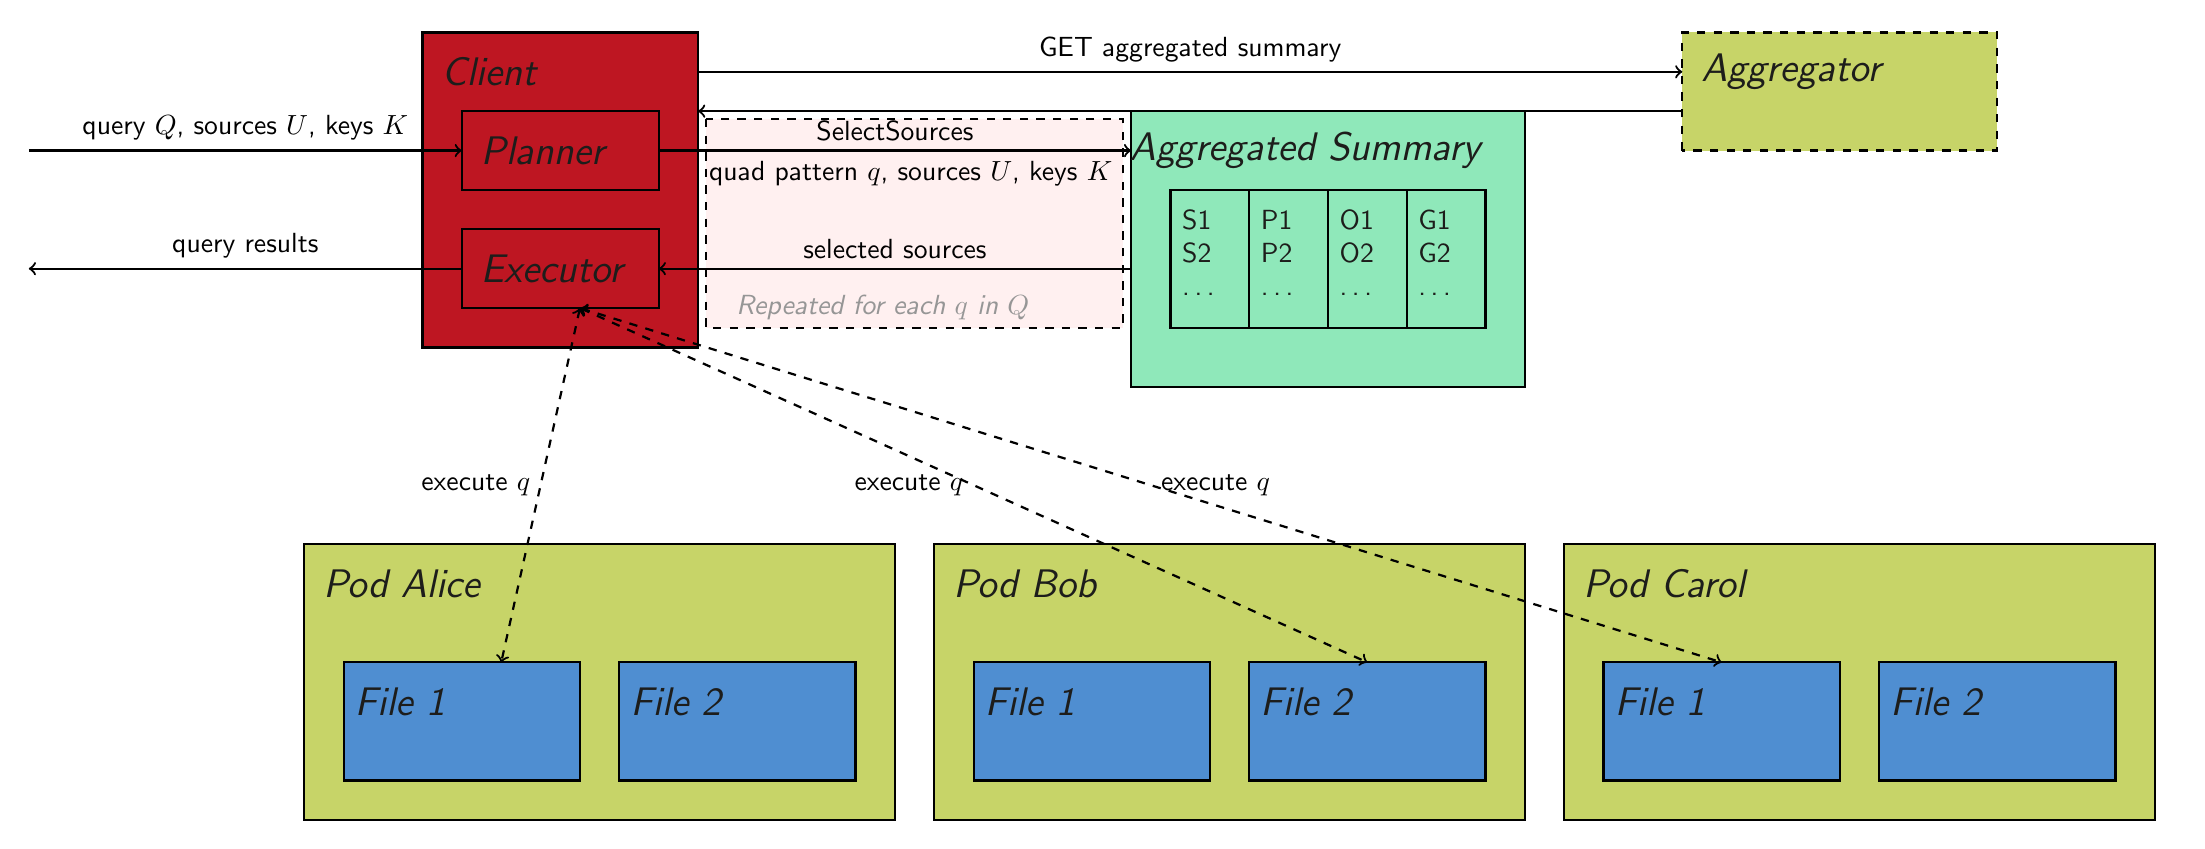
\begin{tikzpicture}[
    node distance = 10em, auto, thick,
    title/.style={text=colortext,font={\Large\itshape}},
    person/.style={text=colorwhite,font={\Large\bfseries}},
    code/.style={text=colortext,font={}},
    key/.style={text=colorkey,font={\tiny\itshape}}
]

    % Client
    \draw[fill=colorclient] (0,0) rectangle (3.5,4);
    \node[title,text width=10em] at (2,3.5) {Client};
    \draw[fill=colorclient] (0.5,2) rectangle (3,3);
    \node[title,text width=10em] at (2.5,2.5) {Planner};
    \draw[fill=colorclient] (0.5,0.5) rectangle (3,1.5);
    \node[title,text width=10em] at (2.5,1) {Executor};
    
    % Arrows to/from client
    \draw[->,thick] (-5,2.5) -- node[midway]{query $Q$, sources $U$, keys $K$} (0.5,2.5);
    \draw[<-,thick] (-5,1) -- node[midway]{query results} (0.5,1);
    
    % Aggregator
    \draw[fill=colorpod,dashed] (16,2.5) rectangle (20,4);
    \node[title,text width=10em] at (18,3.5) {Aggregator};
    
    % Summary
    \draw[fill=colorsummary] (9,3) rectangle (14,-0.5);
    \node[title,text width=20em] at (12.5, 2.5) {Aggregated Summary};
    \draw[fill=colorsummary] (9.5,2) rectangle (10.5,0.25);
    \node[code,text width=2em] at (10,1.2) {S1\\S2\\\ldots};
    \draw[fill=colorsummary] (10.5,2) rectangle (11.5,0.25);
    \node[code,text width=2em] at (11,1.2) {P1\\P2\\\ldots};
    \draw[fill=colorsummary] (11.5,2) rectangle (12.5,0.25);
    \node[code,text width=2em] at (12,1.2) {O1\\O2\\\ldots};
    \draw[fill=colorsummary] (12.5,2) rectangle (13.5,0.25);
    \node[code,text width=2em] at (13,1.2) {G1\\G2\\\ldots};
    
    % Arrows to/from aggregator
    \draw[->,thick] (3.5,3.5) -- node[midway]{GET aggregated summary} (16,3.5);
    \draw[<-,thick] (3.5,3) -- (16,3);
    
    % Repetition
    \draw[dashed,fill=colorrepeat] (3.6,2.9) rectangle (8.9,0.25);
    \node[text width=20em,text=colorgray] at (7.5, 0.5) {\emph{Repeated for each $q$ in $Q$}};
    
    % Arrows between client and summary
    \draw[->,thick] (3,2.5) -- node[above]{SelectSources} node[below,xshift=0.2cm]{quad pattern $q$, sources $U$, keys $K$} (9,2.5);
    \draw[<-,thick] (3,1) -- node[above]{selected sources} (9,1);
    
    % Pod Alice
    \draw[fill=colorpod] (-1.5,-6) rectangle (6,-2.5);
    \node[title,text width=10em] at (0.5,-3) {Pod Alice};
    \draw[fill=colorfile] (-1,-5.5) rectangle (2,-4);
    \node[title,text width=10em] at (0.9,-4.5) {File 1};
    \draw[fill=colorfile] (2.5,-5.5) rectangle (5.5,-4);
    \node[title,text width=10em] at (4.4,-4.5) {File 2};
    
    % Pod Bob
    \draw[fill=colorpod] (6.5,-6) rectangle (14,-2.5);
    \node[title,text width=10em] at (8.5,-3) {Pod Bob};
    \draw[fill=colorfile] (7,-5.5) rectangle (10,-4);
    \node[title,text width=10em] at (8.9,-4.5) {File 1};
    \draw[fill=colorfile] (10.5,-5.5) rectangle (13.5,-4);
    \node[title,text width=10em] at (12.4,-4.5) {File 2};
    
    % Pod Carol
    \draw[fill=colorpod] (14.5,-6) rectangle (22,-2.5);
    \node[title,text width=10em] at (16.5,-3) {Pod Carol};
    \draw[fill=colorfile] (15,-5.5) rectangle (18,-4);
    \node[title,text width=10em] at (16.9,-4.5) {File 1};
    \draw[fill=colorfile] (18.5,-5.5) rectangle (21.5,-4);
    \node[title,text width=10em] at (20.4,-4.5) {File 2};
    
    % Arrows between executor and files
    \draw[<->,thick,dashed] (2,0.5) -- node[left]{execute $q$} (1,-4);
    \draw[<->,thick,dashed] (2,0.5) -- node[left]{execute $q$} (12,-4);
    \draw[<->,thick,dashed] (2,0.5) -- node[right]{execute $q$} (16.5,-4);

\end{tikzpicture}
\end{document}
